%!TEX root = ../main.tex
\chapter{Methodik}
\label{ch:methodik}

Dieses Kapitel beschreibt das methodische Vorgehen bei der Entwicklung des Webshops. Ausgehend vom gewählten iterativ-inkrementellen Vorgehensmodell werden die erhobenen funktionalen und nicht-funktionalen Anforderungen systematisch dokumentiert, bevor die daraus abgeleitete Konzeption und Architektur der Anwendung vorgestellt wird. Die hier getroffenen Entscheidungen folgen etablierten Prinzipien des Software Engineerings und sind auf die spezifischen Rahmenbedingungen einer akademischen Studienarbeit abgestimmt.

\section{Vorgehensmodell}
\label{sec:vorgehensmodell}

\subsection{Auswahl des Vorgehensmodells}
\label{subsec:vorgehensmodell-auswahl}

Für die Entwicklung des Webshops wurde ein iterativ-inkrementelles Vorgehensmodell gewählt, das Elemente aus agilen Methoden mit einer strukturierten Projektplanung verbindet. Die iterativ-inkrementelle Entwicklung (IID) beschreibt Ansätze, bei denen das System schrittweise durch aufeinanderfolgende Iterationen wächst und jede Iteration ein lauffähiges Inkrement liefert \cite{larman2003}. Im Unterschied zu rein plan-getriebenen Modellen wie dem Wasserfallmodell ermöglichen iterative Ansätze frühzeitige Feedbackschleifen und eine kontinuierliche Qualitätssicherung \cite{yadav2015}.

Die Wahl dieses Modells ergab sich aus den konkreten Rahmenbedingungen der Studienarbeit: Das Projekt wurde von zwei Studenten über einen Zeitraum von 36 Wochen neben dem Studium durchgeführt. Ein vollständig agiles Vorgehen wie Scrum war daher nicht sinnvoll, da es einen dedizierten Product Owner und regelmäßige Sprint-Reviews mit externen Stakeholdern voraussetzt \cite{yadav2015}. Stattdessen wurde ein schlanker, meilensteinbasierter Ansatz gewählt, der klare Zwischenziele definiert und gleichzeitig Spielraum für iterative Anpassungen lässt.

Weitere Entscheidungsfaktoren waren die technologische Unsicherheit beim Einstieg in Firebase als Backend-as-a-Service-Plattform \cite{uunonen2023} sowie die weitgehend stabilen Anforderungen an einen B2C-Webshop, die eine vorausschauende Planung ermöglichten \cite{heinemann2024}.

\subsection{Projektphasen}
\label{subsec:projektphasen}

Das Projekt wurde in acht Meilensteine gegliedert, die über einen Zeitraum von 36 Wochen bearbeitet wurden:

\begin{figure}[h]
    \centering
    
\includegraphics[width=1\textwidth]{meilenstein.png}
    \caption{Meilensteine und Zeitplan der Projektphasen}
    \label{fig:meilensteine}
\end{figure}

Die Meilensteine orientieren sich am Prinzip der inkrementellen Systemerweiterung, bei der jede Phase auf den Ergebnissen der vorherigen aufbaut und ein funktional erweitertes Inkrement liefert \cite{larman2003}. Die ersten Phasen umfassten die Anforderungsanalyse sowie die Einrichtung der Entwicklungsumgebung einschließlich Firebase-Projektkonfiguration und Versionsverwaltung mit Git. In den mittleren Meilensteinen wurden die Kernkomponenten des Webshops realisiert -- zunächst Produktverwaltung und Benutzerauthentifizierung, da diese die funktionalen Voraussetzungen aller nachfolgenden Komponenten darstellen. Beispielsweise setzt der Warenkorb eine funktionierende Produktansicht voraus, und der Checkout-Prozess erfordert ein implementiertes Authentifizierungssystem. Die abschließenden Phasen widmeten sich dem Angebotssystem, der Administrationsoberfläche sowie dem systematischen Testing und der Deployment-Vorbereitung.

\section{Anforderungsanalyse}
\label{sec:anforderungsanalyse}

Die Anforderungsanalyse ist eine zentrale Disziplin des Software Engineerings und bildet die Grundlage für die gesamte Systementwicklung. Sie zielt auf eine vollständige, konsistente und verifizierbare Beschreibung aller Systemeigenschaften aus Nutzersicht ab und schafft damit die Basis für Entwurf, Implementierung und Qualitätssicherung. Grundlegend wird zwischen \textit{funktionalen Anforderungen}, die beschreiben \textit{was} das System leisten soll, und \textit{nicht-funktionalen Anforderungen}, die beschreiben \textit{wie} das System seine Aufgaben erfüllen soll, unterschieden. Für E-Commerce-Systeme ist diese Unterscheidung von besonderer Relevanz, da neben der Funktionalität insbesondere Qualitätsmerkmale wie Performance, Sicherheit und Benutzerfreundlichkeit maßgeblich über Nutzerakzeptanz und wirtschaftlichen Erfolg der Anwendung entscheiden \cite{garcialopez2020}.

\subsection{Funktionale Anforderungen}
\label{subsec:funktionale-anforderungen}

Die funktionalen Anforderungen wurden auf Basis einer Analyse typischer E-Commerce-Systeme sowie der in der Disposition definierten Projektziele erhoben \cite{heinemann2024, garcialopez2020}. Zur strukturierten Priorisierung wurde das MoSCoW-Verfahren eingesetzt: \textit{Muss}-Anforderungen sind für die Grundfunktionalität zwingend erforderlich, \textit{Soll}-Anforderungen sind bedeutsam aber nicht zwingend, und \textit{Kann}-Anforderungen sind wünschenswert, ohne das Projektziel zu gefährden.

\subsubsection{Benutzerverwaltung}

Die Benutzerverwaltung umfasst alle Funktionen zur Registrierung, Anmeldung und Kontoverwaltung. Da der Webshop personalisierte Features wie gespeicherte Adressen und eine Bestellhistorie anbietet, ist eine zuverlässige Identitätsverwaltung eine zentrale Voraussetzung für den Betrieb. Die Passwort-Zurücksetzen-Funktion (FA-03) sowie die DSGVO-konforme Kontolöschung (FA-06) wurden ebenfalls aufgenommen, da sie für einen produktionsreifen Shop erwartet werden.

\begin{table}[H]
\centering
\begin{tabularx}{\textwidth}{|c|X|c|}
\hline
\textbf{ID} & \textbf{Anforderung} & \textbf{Priorität} \\
\hline
FA-01 & Benutzer können sich mit E-Mail und Passwort registrieren & Muss \\
\hline
FA-02 & Benutzer können sich anmelden und abmelden & Muss \\
\hline
FA-03 & Benutzer können ihr Passwort zurücksetzen & Muss \\
\hline
FA-04 & Benutzer können ihre Profildaten einsehen und bearbeiten & Muss \\
\hline
FA-05 & Benutzer können ihre Bestellhistorie einsehen & Muss \\
\hline
FA-06 & Benutzer können ihr Konto löschen & Soll \\
\hline
\end{tabularx}
\caption{Funktionale Anforderungen: Benutzerverwaltung}
\label{tab:fa-benutzer}
\end{table}

\subsubsection{Produktkatalog}

Der Produktkatalog bildet den inhaltlichen Kern des Webshops. Die Anforderungen adressieren sowohl die Darstellung einzelner Produkte als auch die Navigation und Suche, da diese Funktionen direkt die Nutzerführung zum Kauf beeinflussen \cite{heinemann2024}. Die Wunschliste (FA-16) wurde bewusst als optionale \textit{Kann}-Anforderung eingestuft, da sie keinen direkten Einfluss auf den Kaufprozess hat.

\begin{table}[H]
\centering
\begin{tabularx}{\textwidth}{|c|X|c|}
\hline
\textbf{ID} & \textbf{Anforderung} & \textbf{Priorität} \\
\hline
FA-10 & Produkte werden mit Bild, Titel, Beschreibung und Preis angezeigt & Muss \\
\hline
FA-11 & Produkte sind in Kategorien organisiert & Muss \\
\hline
FA-12 & Benutzer können Produkte nach Kategorien filtern & Muss \\
\hline
FA-13 & Benutzer können Produkte über eine Suchfunktion finden & Muss \\
\hline
FA-14 & Die Verfügbarkeit von Produkten wird angezeigt & Muss \\
\hline
FA-15 & Benutzer können Produktdetails auf einer separaten Seite ansehen & Soll \\
\hline
FA-16 & Benutzer können Produkte auf eine Wunschliste setzen & Kann \\
\hline
\end{tabularx}
\caption{Funktionale Anforderungen: Produktkatalog}
\label{tab:fa-produkte}
\end{table}

\subsubsection{Warenkorb und Bestellung}

Warenkorb und Bestellprozess sind die transaktionskritischen Komponenten des Webshops und decken den vollständigen Kauffluss von der Produktauswahl bis zur Bestellbestätigung ab. Empirische Studien zeigen, dass ein reibungsloser Checkout-Prozess maßgeblich die Abbruchrate beeinflusst \cite{butnampetch2020}. Die browserübergreifende Persistenz des Warenkorbs (FA-27) verbessert die Nutzererfahrung bei wiederkehrenden Besuchern und wurde daher als \textit{Soll}-Anforderung aufgenommen.

\begin{table}[H]
\centering
\begin{tabularx}{\textwidth}{|c|X|c|}
\hline
\textbf{ID} & \textbf{Anforderung} & \textbf{Priorität} \\
\hline
FA-20 & Benutzer können Produkte zum Warenkorb hinzufügen & Muss \\
\hline
FA-21 & Benutzer können die Menge im Warenkorb ändern & Muss \\
\hline
FA-22 & Benutzer können Produkte aus dem Warenkorb entfernen & Muss \\
\hline
FA-23 & Der Warenkorb zeigt Zwischensumme und Gesamtpreis & Muss \\
\hline
FA-24 & Angemeldete Benutzer können den Checkout-Prozess starten & Muss \\
\hline
FA-25 & Im Checkout werden Lieferadresse und Zahlungsart erfasst & Muss \\
\hline
FA-26 & Nach Bestellabschluss erhält der Benutzer eine Bestätigung & Muss \\
\hline
FA-27 & Der Warenkorb bleibt auch nach Schließen des Browsers erhalten & Soll \\
\hline
\end{tabularx}
\caption{Funktionale Anforderungen: Warenkorb und Bestellung}
\label{tab:fa-warenkorb}
\end{table}

\subsubsection{Angebotssystem}

Das Angebotssystem ermöglicht zeitlich begrenzte Rabattaktionen und ist ein typisches Werkzeug moderner E-Commerce-Plattformen zur Kundenbindung \cite{heinemann2024}. Da die Funktion inhaltlich auf einem funktionierenden Produktkatalog und Warenkorb aufbaut, wurden alle zugehörigen Anforderungen als \textit{Soll} priorisiert -- sie erweitern den Shop sinnvoll, sind aber nicht für den Grundbetrieb notwendig.

\begin{table}[H]
\centering
\begin{tabularx}{\textwidth}{|c|X|c|}
\hline
\textbf{ID} & \textbf{Anforderung} & \textbf{Priorität} \\
\hline
FA-30 & Administratoren können zeitlich begrenzte Angebote erstellen & Soll \\
\hline
FA-31 & Angebote können prozentuale oder absolute Rabatte definieren & Soll \\
\hline
FA-32 & Aktive Angebote werden auf der Startseite hervorgehoben & Soll \\
\hline
FA-33 & Rabatte werden automatisch im Warenkorb angewendet & Soll \\
\hline
\end{tabularx}
\caption{Funktionale Anforderungen: Angebotssystem}
\label{tab:fa-angebote}
\end{table}

\subsubsection{Administration}

Der Administrationsbereich stellt die Verwaltungsoberfläche für den Shopbetreiber bereit. Produktpflege, Kategorieverwaltung und Bestellstatus-Management (FA-41 bis FA-44) sind als \textit{Muss}-Anforderungen definiert, da ohne sie kein laufender Betrieb des Shops möglich wäre. Der Zugang zum Administrationsbereich ist auf Benutzer mit Admin-Rolle beschränkt (FA-40), was direkte Auswirkungen auf das Sicherheits- und Berechtigungskonzept hat.

\begin{table}[H]
\centering
\begin{tabularx}{\textwidth}{|c|X|c|}
\hline
\textbf{ID} & \textbf{Anforderung} & \textbf{Priorität} \\
\hline
FA-40 & Der Administrationsbereich ist durch Authentifizierung geschützt & Muss \\
\hline
FA-41 & Administratoren können Produkte erstellen, bearbeiten und löschen & Muss \\
\hline
FA-42 & Administratoren können Kategorien verwalten & Muss \\
\hline
FA-43 & Administratoren können Bestellungen einsehen und deren Status ändern & Muss \\
\hline
FA-44 & Administratoren können Lagerbestände aktualisieren & Muss \\
\hline
FA-45 & Administratoren können Benutzerkonten einsehen und löschen & Soll \\
\hline
FA-46 & Administratoren können Angebote erstellen und verwalten & Soll \\
\hline
\end{tabularx}
\caption{Funktionale Anforderungen: Administration}
\label{tab:fa-admin}
\end{table}

\subsection{Nicht-funktionale Anforderungen}
\label{subsec:nichtfunktionale-anforderungen}

Nicht-funktionale Anforderungen definieren die Qualitätsmerkmale des Systems und legen fest, unter welchen Bedingungen und mit welcher Güte die funktionalen Anforderungen erfüllt werden müssen \cite{garcialopez2020}. Sie umfassen Aspekte wie Performance, Sicherheit, Kompatibilität und Wartbarkeit und beeinflussen maßgeblich Architekturentscheidungen und Technologieauswahl. Besonders die Ladezeit-Anforderung (NFA-01) und die Responsive-Design-Anforderung (NFA-03) haben direkten Einfluss auf die Nutzerzufriedenheit und Conversion-Rate im E-Commerce \cite{peterson2018}.

\begin{table}[H]
\centering
\begin{tabularx}{\textwidth}{|c|X|c|}
\hline
\textbf{ID} & \textbf{Anforderung} & \textbf{Kategorie} \\
\hline
NFA-01 & Die Anwendung lädt initial innerhalb von 3 Sekunden & Performance \\
\hline
NFA-02 & Die Anwendung funktioniert auf aktuellen Versionen von Chrome, Firefox, Safari und Edge & Kompatibilität \\
\hline
NFA-03 & Die Anwendung ist auf Bildschirmen von 320px bis 2560px Breite nutzbar & Responsivität \\
\hline
NFA-04 & Alle Datenübertragungen erfolgen verschlüsselt (HTTPS) & Sicherheit \\
\hline
NFA-05 & Passwörter werden gemäß aktueller Standards gehasht gespeichert & Sicherheit \\
\hline
NFA-06 & Die Anwendung entspricht den Anforderungen der DSGVO & Compliance \\
\hline
NFA-07 & Der Code folgt einheitlichen Formatierungs- und Namenskonventionen & Wartbarkeit \\
\hline
NFA-08 & Die Anwendung ist ohne JavaScript-Kenntnisse bedienbar & Benutzerfreundlichkeit \\
\hline
\end{tabularx}
\caption{Nicht-funktionale Anforderungen}
\label{tab:nfa}
\end{table}

\subsection{Abgrenzung}
\label{subsec:abgrenzung}

Zur Eingrenzung des Projektumfangs auf die Kernfunktionalitäten eines E-Commerce-Systems wurden bewusst bestimmte Funktionalitäten ausgeschlossen. Diese Priorisierung folgt dem Prinzip der inkrementellen Systementwicklung, bei der zunächst ein stabiler funktionaler Kern realisiert wird, bevor optionale Erweiterungen in Betracht gezogen werden \cite{larman2003}:

\begin{itemize}
    \item \textbf{Echte Zahlungsabwicklung:} Die Integration eines Zahlungsdienstleisters wie PayPal oder Stripe ist nicht Teil des Prototyps. Der Checkout-Prozess simuliert die Zahlungserfassung.
    
    \item \textbf{Versandintegration:} Eine Anbindung an Versanddienstleister zur Sendungsverfolgung ist nicht vorgesehen.
    
    \item \textbf{Mehrsprachigkeit:} Die Anwendung wird ausschließlich in deutscher Sprache entwickelt.
    
    \item \textbf{Produktbewertungen:} Ein System für Kundenbewertungen und -rezensionen ist nicht Teil des Projektumfangs.
    
    \item \textbf{Newsletter:} Eine Newsletter-Funktionalität mit E-Mail-Marketing ist nicht vorgesehen.
\end{itemize}

Diese Abgrenzungen spiegeln den Charakter der Arbeit als funktionalen Prototyp wider: Der Webshop demonstriert alle wesentlichen Abläufe eines B2C-Onlineshops, ohne den Rahmen einer Studienarbeit zu überschreiten.

\section{Konzeption und Architektur}
\label{sec:konzeption-architektur}

Auf Basis der erhobenen Anforderungen wurde die Architektur des Webshops konzipiert. Die zentralen Entwurfsentscheidungen -- Systemarchitektur, Datenbankstruktur, Frontend-Komponentenmodell und Sicherheitskonzept -- werden in diesem Abschnitt erläutert und begründet.

\subsection{Systemarchitektur}
\label{subsec:systemarchitektur}

Die Anwendung folgt einer Client-Server-Architektur, bei der das Frontend als Single Page Application im Browser des Benutzers ausgeführt wird und über wohldefinierte APIs mit den Firebase-Backend-Diensten kommuniziert. Dieses Architekturmuster ermöglicht eine klare Trennung von Präsentationslogik und Datenhaltung und bildet die Grundlage für eine unabhängige Weiterentwicklung beider Schichten \cite{newman2021}.

\begin{figure}[H]
\centering
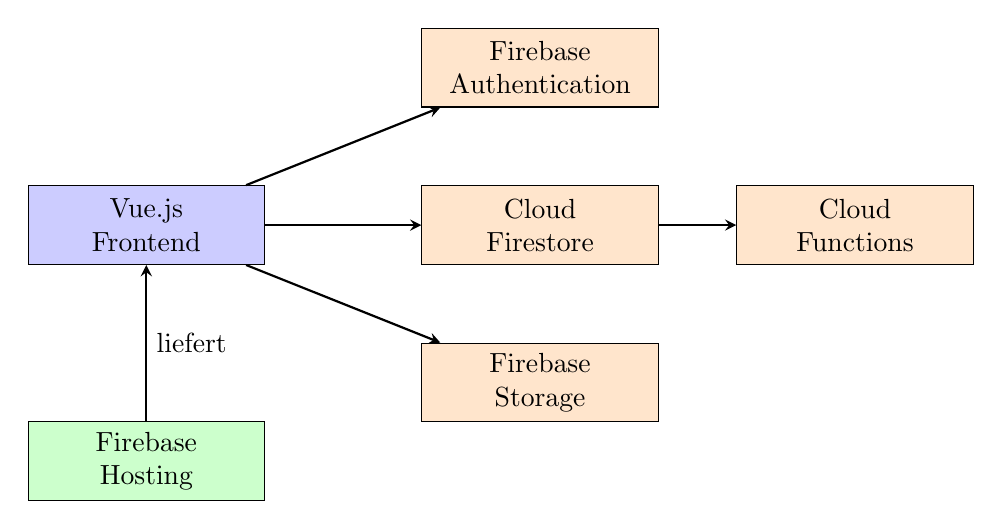
\begin{tikzpicture}[
    box/.style={rectangle, draw, minimum width=3cm, minimum height=1cm, align=center},
    arrow/.style={->, >=stealth, thick}
]
    % Client
    \node[box, fill=blue!20] (client) at (0,0) {Vue.js\\Frontend};
    
    % Firebase Services
    \node[box, fill=orange!20] (auth) at (5,2) {Firebase\\Authentication};
    \node[box, fill=orange!20] (firestore) at (5,0) {Cloud\\Firestore};
    \node[box, fill=orange!20] (storage) at (5,-2) {Firebase\\Storage};
    \node[box, fill=orange!20] (functions) at (9,0) {Cloud\\Functions};
    
    % Hosting
    \node[box, fill=green!20] (hosting) at (0,-3) {Firebase\\Hosting};
    
    % Arrows
    \draw[arrow] (client) -- (auth);
    \draw[arrow] (client) -- (firestore);
    \draw[arrow] (client) -- (storage);
    \draw[arrow] (firestore) -- (functions);
    \draw[arrow] (hosting) -- (client) node[midway, right] {liefert};
    
\end{tikzpicture}
\caption{Systemarchitektur des Webshops}
\label{fig:systemarchitektur}
\end{figure}

Die Architektur zeichnet sich durch folgende Merkmale aus:

\textbf{Lose Kopplung:} Frontend und Backend-Dienste kommunizieren ausschließlich über definierte APIs. Dieses Prinzip ermöglicht die unabhängige Weiterentwicklung und den Austausch einzelner Systemkomponenten ohne kaskadierende Auswirkungen auf andere Teile des Systems \cite{newman2021}.

\textbf{Zustandslosigkeit:} Der Server speichert keinen Client-Zustand zwischen Anfragen. Session-Informationen werden im Client verwaltet, und Authentifizierungstoken werden bei jeder Anfrage mitgesendet. Zustandslose Dienste lassen sich ohne Replika-Synchronisation horizontal skalieren und sind damit ein Grundprinzip moderner, hochverfügbarer Webarchitekturen.

\textbf{Ereignisgesteuert:} Änderungen in der Datenbank können Cloud Functions auslösen, die serverseitige Logik ausführen. Dieses reaktive Verarbeitungsmodell ohne aktives Polling ist ein charakteristisches Merkmal serverloser Architekturen und ermöglicht eine ressourcenschonende, bedarfsgesteuerte Ausführung von Backend-Logik \cite{shafiei2022}.

\subsection{Datenbankstruktur}
\label{subsec:datenbankstruktur}

Cloud Firestore ist eine dokumentenorientierte NoSQL-Datenbank, die Daten in Dokumenten und Collections organisiert \cite{kesavan2023}. Im Unterschied zu relationalen Datenbanken erlaubt dieses schemalose Modell eine flexible Datenstrukturierung, die sich besonders für die hierarchisch organisierten Datenobjekte eines Webshops eignet. Für den Webshop wurden folgende Haupt-Collections definiert:

\textbf{users:} Speichert Benutzerdaten wie Name, E-Mail, Adresse und Rolle. Die Dokument-ID entspricht der Firebase Auth UID.

\textbf{products:} Enthält alle Produktinformationen einschließlich Name, Beschreibung, Preis, Kategorie und Lagerbestand. Produktbilder werden als URLs zu Firebase Storage gespeichert.

\textbf{categories:} Definiert die verfügbaren Produktkategorien mit Name und optionaler Beschreibung.

\textbf{orders:} Speichert Bestellungen mit Referenz zum Benutzer, bestellten Produkten, Gesamtbetrag, Lieferadresse und Bestellstatus.

\textbf{offers:} Enthält Sonderangebote mit Gültigkeitszeitraum, Rabatttyp und -höhe sowie Referenzen zu betroffenen Produkten.

\begin{figure}[H]
\centering
\begin{tikzpicture}[
    collection/.style={rectangle, draw, fill=blue!10, minimum width=2.5cm, minimum height=0.8cm},
    field/.style={rectangle, draw, fill=gray!10, minimum width=2.5cm, minimum height=0.5cm, font=\small},
    arrow/.style={->, >=stealth}
]
    % Users Collection
    \node[collection] (users) at (0,0) {users};
    \node[field, below=0.1cm of users] (u1) {email};
    \node[field, below=0.1cm of u1] (u2) {displayName};
    \node[field, below=0.1cm of u2] (u3) {role};
    \node[field, below=0.1cm of u3] (u4) {address};
    
    % Products Collection
    \node[collection] (products) at (4,0) {products};
    \node[field, below=0.1cm of products] (p1) {name};
    \node[field, below=0.1cm of p1] (p2) {price};
    \node[field, below=0.1cm of p2] (p3) {categoryId};
    \node[field, below=0.1cm of p3] (p4) {stock};
    
    % Orders Collection
    \node[collection] (orders) at (8,0) {orders};
    \node[field, below=0.1cm of orders] (o1) {userId};
    \node[field, below=0.1cm of o1] (o2) {items[]};
    \node[field, below=0.1cm of o2] (o3) {total};
    \node[field, below=0.1cm of o3] (o4) {status};
    
    % Categories Collection
    \node[collection] (categories) at (4,-4) {categories};
    \node[field, below=0.1cm of categories] (c1) {name};
    \node[field, below=0.1cm of c1] (c2) {description};
    
    % Relationships
    \draw[arrow, dashed] (p3.south) -- (categories.north);
    \draw[arrow, dashed] (o1.west) -- +(-1,0) |- (users.east);
    
\end{tikzpicture}
\caption{Vereinfachtes Datenbankschema}
\label{fig:datenbankschema}
\end{figure}

\subsection{Frontend-Komponentenarchitektur}
\label{subsec:komponentenarchitektur}

Das Frontend ist nach dem Komponentenprinzip von Vue.js strukturiert. Komponentenbasierte Architektur hat sich als dominantes Paradigma in der modernen Frontend-Entwicklung etabliert, da sie Wiederverwendbarkeit, Testbarkeit und eine klare Trennung von Verantwortlichkeiten fördert \cite{kothapalli2021}. Die Komponenten sind hierarchisch organisiert und nach ihrer Funktion gruppiert:

\textbf{Views:} Seitenkomponenten, die über den Router angesteuert werden. Sie entsprechen den Hauptseiten der Anwendung wie Startseite, Produktübersicht oder Checkout.

\textbf{Layout-Komponenten:} Strukturelle Komponenten wie Header, Footer und Navigation, die auf mehreren Seiten verwendet werden.

\textbf{Feature-Komponenten:} Fachliche Komponenten wie Produktkarte, Warenkorb-Dialog oder Bestellübersicht, die spezifische Funktionalitäten kapseln.

\textbf{Utility-Komponenten:} Wiederverwendbare UI-Elemente wie Buttons, Eingabefelder oder Benachrichtigungen.

Die Kommunikation zwischen Komponenten erfolgt über:

\begin{itemize}
    \item \textbf{Props:} Datenübergabe von Eltern- an Kind-Komponenten
    \item \textbf{Events:} Kommunikation von Kind- zu Eltern-Komponenten
    \item \textbf{Stores:} Zentraler Zustand für komponentenübergreifende Daten (Pinia)
\end{itemize}

\subsection{Sicherheitskonzept}
\label{subsec:sicherheitskonzept}

Die Sicherheit der Anwendung basiert auf einem mehrschichtigen Sicherheitskonzept (\textit{Defense in Depth}), das Schutzmaßnahmen auf verschiedenen Ebenen des Systems kombiniert. Dieses Prinzip stellt sicher, dass das Kompromittieren einer einzelnen Schutzmaßnahme nicht zur vollständigen Kompromittierung des Systems führt, und entspricht den Empfehlungen der OWASP für moderne Webanwendungen \cite{fredj2020}:

\textbf{Authentifizierung:} Firebase Authentication verwaltet die Benutzeridentität und implementiert OAuth~2.0-kompatible Authentifizierungsabläufe. Bei erfolgreicher Anmeldung erhält der Client ein JSON Web Token (JWT) -- ein kryptographisch signiertes, selbst-beschreibendes Token mit begrenzter Gültigkeitsdauer, das bei allen Backend-Anfragen im Authorization-Header mitgesendet wird \cite{bucko2023}.

\textbf{Autorisierung:} Firestore Security Rules definieren deklarativ, welche authentifizierten Benutzer auf welche Daten zugreifen und welche Operationen sie ausführen dürfen. Diese serverseitige Durchsetzung stellt sicher, dass Zugriffskontrollen nicht durch clientseitige Manipulationen umgangen werden können \cite{firestore2025}. Beispielsweise können Benutzer ausschließlich ihre eigenen Bestellungen lesen, während Administratoren Zugriff auf alle Collections haben.

\textbf{Datenverschlüsselung:} Alle Kommunikation zwischen Client und Firebase erfolgt über HTTPS mit TLS-Verschlüsselung. Firebase verschlüsselt darüber hinaus alle gespeicherten Daten automatisch, sodass die Anforderung NFA-04 ohne zusätzlichen Implementierungsaufwand erfüllt wird.

\textbf{Input-Validierung:} Benutzereingaben werden sowohl im Frontend als auch durch Firestore Security Rules im Backend validiert, um Injection-Angriffe und fehlerhafte Datenzustände zu verhindern \cite{fredj2020}.

Ein Beispiel für Firestore Security Rules:

\begin{lstlisting}[language=Java, caption=Firestore Security Rules (Auszug)]
rules_version = '2';
service cloud.firestore {
  match /databases/{database}/documents {
    // Benutzer koennen nur eigene Daten lesen/schreiben
    match /users/{userId} {
      allow read, write: if request.auth != null 
                         && request.auth.uid == userId;
    }
    
    // Produkte sind oeffentlich lesbar
    match /products/{productId} {
      allow read: if true;
      allow write: if isAdmin();
    }
    
    // Hilfsfunktion zur Admin-Pruefung
    function isAdmin() {
      return request.auth != null 
             && get(/databases/$(database)/documents/users/$(request.auth.uid)).data.role == 'admin';
    }
  }
}
\end{lstlisting}

\subsection{Deployment-Konzept}
\label{subsec:deployment-konzept}

Das Deployment der Anwendung erfolgt über Firebase Hosting mit automatisierter CI/CD-Pipeline (Continuous Integration~/ Continuous Deployment). Automatisierte Deployment-Pipelines reduzieren manuelle Fehlerquellen und stellen sicher, dass ausschließlich getesteter und verifizierter Code in die Produktionsumgebung gelangt \cite{chacon2014}.

\begin{enumerate}
    \item \textbf{Build:} Der Vue.js-Quellcode wird durch Vite zu optimierten statischen Dateien kompiliert.
    \item \textbf{Test:} Automatisierte Tests prüfen die Funktionalität der Anwendung.
    \item \textbf{Deploy:} Die Build-Artefakte werden zu Firebase Hosting hochgeladen.
    \item \textbf{Aktivierung:} Firebase aktiviert die neue Version und routet Traffic automatisch um.
\end{enumerate}

Firebase Hosting bietet dabei Features wie automatische SSL-Zertifikate, globales CDN und atomare Deployments mit Rollback-Möglichkeit.
